\begin{center}
\textsc{\Large Laboratorio 14}~\\
{\large Videojuegos, Físicas, Programación}~\\
\emph{Física en Videojuegos, Partículas y Proyectiles}
\end{center}

\section{Pre-Laboratorio}
\begin{itemize}
\item Investigar:
\begin{enumerate}
  \item Movimiento parabólico y rectilíneo y rectilíneo uniforme.
  \item Definición de partícula.
  \item Simulación N-Body y Simulación Barnes-Hut.
\end{enumerate}
\item De algún juego que conozca analice.
\begin{enumerate}
  \item ¿En este juego existe el uso de proyectiles o partículas? 
  \item Si el juego posee ¿cual cree que sea el propósito de estas partículas y/o proyectiles?
  \item En caso de no tener ¿considera algún caso donde el juego se pueda beneficiar de agregar partículas o proyectiles?
\end{enumerate}
\end{itemize}

\section{Introducción}
Para agregar realismo, nuevas mecánicas o mayor calidad visual se introducen leyes físicas dentro del motor de juego, es mayormente usado en juegos tridimensionales \cite[p.~325]{jenkinscreatinggames}. Estas nuevos efectos se introducen en forma de simulaciones las cuales son aproximaciones de fenómenos reales utilizando valores discretos \cite{ian_gamephysics}. En el ambiente de un videojuegos una simulación completa y totalmente correcta podría causar complicaciones en las mecánicas de juego, progreso de la historia o hacer tediosas ciertas actividades.

\section{Sistemas de Partículas}
\setlength\intextsep{0pt}
\begin{wrapfigure}[10]{r}{0.35\linewidth}
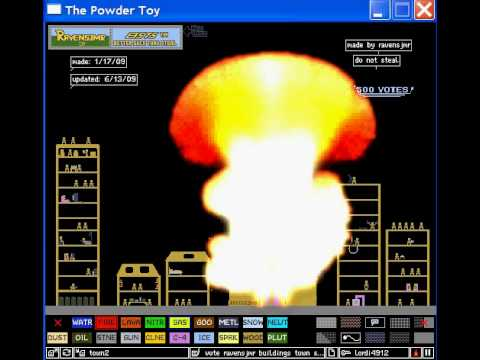
\includegraphics[width=\linewidth]{media/powdertoy.jpg}
\caption{\emph{Powder Toy} un juego 2D que utiliza sistemas de particulas.}
\label{fig:particles}
\end{wrapfigure}
Es una técnica utilizada en físicas de juegos y computación gráfica en la que se usa una cantidad grande de pequeños \emph{sprites} u otros objetos visuales para simular ciertos fenómenos como sistemas altamente caóticos, fenómenos naturales o procesos causados por reacciones químicas \cite{vanderburg_particlesystem}. 

Algunos ejemplos de fenómenos que son replicados utilizando sistemas de partículas, es el fuego, explosiones, humo, agua en movimiento (como cascadas de agua), nubes, estrellas, galaxias, etc. Es también común su uso para efectos visuales abstractos.
\section{Proyectiles}
\setlength\intextsep{0pt}
\begin{wrapfigure}[10]{l}{0.4\linewidth}
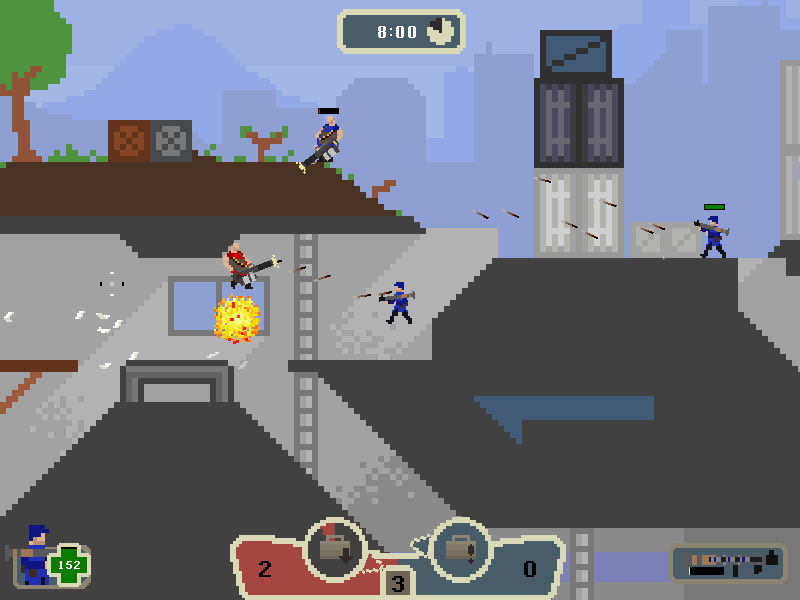
\includegraphics[width=\linewidth]{media/Gang_Garrison_2.png}
\caption{Gang Garrison 2 un shooter 2D basado en Team Fortress 2, distintas clases tienen distintos tipos de proyectiles.}
\label{fig:ganggarrison2}
\end{wrapfigure}

En algunos videojuegos los objetos de tipo proyectil son sometidos a simulaciones físicas o aproximaciones. Usualmente en la programación de un juego un proyectil sigue una linea recta o parabólica y en caso de colisión se inicia algún evento. Otros juegos consideran factores que afectan la trayectoria del proyectil tales como resistencia y/o dirección al viento, velocidad de proyectil (en vez de una trayectoria inmediata el proyectil posee una velocidad en espacio), gravedad, entre otros \cite{fifa_physics}.~\\

\section{Actividad}
Durante esta actividad se busca agregar físicas al juego para mejorar la inmersión y calidad visual del juego. Este laboratorio se enfocara en el uso de simulaciones físicas con el uso de sistemas de partículas.
\begin{itemize}
\item Se debe hacer uso de sistemas de partículas para varios objetos en escena.
\item Provocar el uso de sistemas de partículas al colisionar un objeto contra otro objeto o proyectil. Esto se puede usar para simular una explosión o cualquier otro efecto visual.
\end{itemize}
